\documentclass[10pt]{article}
\setlength{\topmargin}{-0.5in}
\setlength{\textwidth}{6.5in}
\setlength{\oddsidemargin}{0in}
\setlength{\textheight}{9in}

%\usepackage{multirow}
%\usepackage{rotating}
\usepackage[fleqn]{amsmath}
\usepackage{amsfonts}
\usepackage{natbib}
\usepackage{palatino}
\usepackage{url}
\usepackage{graphicx}

\newcommand{\wlin}{\mathbf{w}_{\text{lin}}}

\begin{document}

\title{CSE 417T: Homework 4 Solution Sketches}

\maketitle

\noindent \textbf{Note:} These are not intended to be comprehensive,
just to help you see what the answers should be.


\begin{enumerate}

\item

  \begin{itemize}
    \item[(a)] The figure of OOB error vs the number of bags would look like the following (there are randomness involved, so as long as the ``shape'' is similar, it's fine.)
      \begin{figure}[h]
        \begin{center}
        \includegraphics[width=.5\textwidth]{oob-vs-numbags.eps}
        \end{center}
      \end{figure}

%    \item[(b)] The cross-validation error for decision trees and the OOB error for the bagging implementation are reported below:
%        \begin{center}
%        \begin{tabular}{l|c|c}
%            & Decision Trees & Bagged Trees \\
%            \hline
%            One-vs-Three & 0.0078 & 0.0036 \\
%            \hline
%            Three-vs-Five & 0.0610 & 0.0395
%        \end{tabular}
%        \end{center}
    \item[(b)] 
        The OOB errors for the bagging implementation are reported below:
        \begin{center}
        \begin{tabular}{l|c}
                & Bagged Trees \\
            \hline
            One-vs-Three & 0.0018 \\
            \hline
            Three-vs-Five & 0.0313
          \end{tabular}
          \end{center}


        The test errors for decision trees and the bagging implementation are reported below:
        \begin{center}
        \begin{tabular}{l|c|c}
                & Decision Trees & Bagged Trees \\
            \hline
            One-vs-Three & 0.0140 & 0.0116 \\
            \hline
            Three-vs-Five & 0.1258 & 0.0798
          \end{tabular}
          \end{center}
    As the number of ensembles goes large, the OOB error decreases. This fits the analysis that the variances for the bagged tree decreases.  
    Three-vs-Five is a harder question.
    OOB error serves as a fine estimation for out-of-sample error.
    %Both OOB and cross-validation error serves as fine estimations for out-of-sample error.
  \end{itemize}



\item
 
(a) The root node of the decision tree after running ID3 is ``Stripe''. 
Let $H(p)= p\log(1/p) + (1-p)\log(1/(1-p))$ be the entropy of binary signals in which one of the signals has probability $p$ in the distribution. 
We can calculate the information gain for choosing each attribute. 

The entropy of the data before splitting is
$\frac{2}{5}\log\left(\frac{5}{2}\right)+\frac{3}{5}\log\left(\frac{5}{3}\right) \approx 0.971$.

The average entropy after splitting using ``Color'' is
$\frac{1}{5} \times 0 + \frac{4}{5} \left[ \frac{2}{4}\log\left(\frac{4}{2}\right) + \frac{2}{4}\log\left(\frac{4}{2}\right)\right] = 0.8$.

The average entropy after splitting using ``Stripes'' is
$\frac{2}{5} \times 0 + \frac{3}{5} \left[ \frac{1}{3}\log\left(\frac{3}{1}\right) + \frac{2}{3}\log\left(\frac{3}{2}\right)\right] \approx 0.551$.

The average entropy after splitting using ``Texture'' is
$\frac{2}{5} \left[\frac{1}{2}\log\left(\frac{2}{1}\right) + \frac{1}{2}\log\left(\frac{2}{1}\right)\right] + \frac{3}{5} \left[ \frac{1}{3}\log\left(\frac{3}{1}\right) + \frac{2}{3}\log\left(\frac{3}{2}\right)\right] \approx 0.951$.

Given the above values, we have
\begin{align*}
Gain(D,\mbox{Color}) &\approx 0.971 - 0.8 = 0.171 \\
Gain(D,\mbox{Stripes}) &\approx 0.971 - 0.551 = 0.420 \\ 
Gain(D,\mbox{Texture}) &\approx 0.971 - 0.951 = 0.020 
\end{align*}
Therefore, splitting using ``Stripes'' leads to the maximum information gain.

(b) The final decision tree looks like the following:
\begin{figure}[h!]
  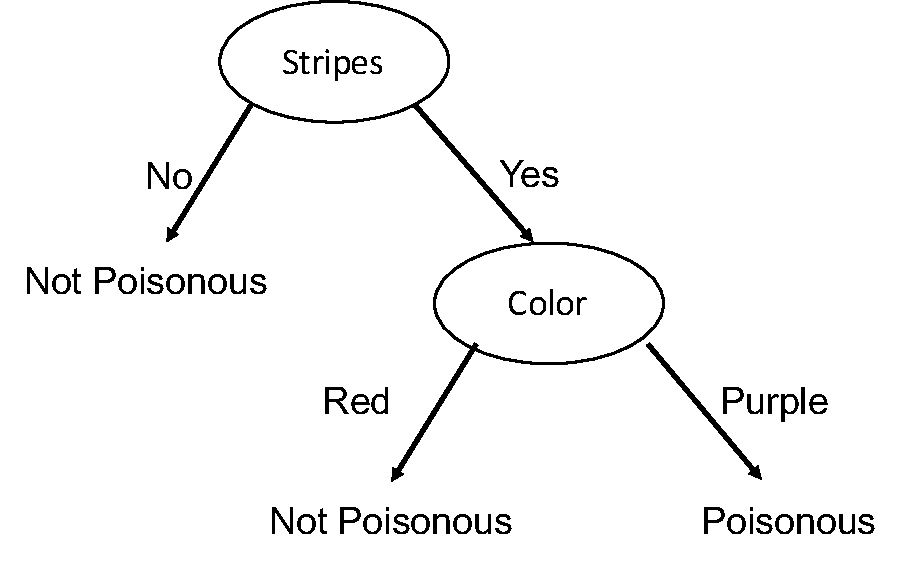
\includegraphics[width=0.45\textwidth]{tree.pdf}
  \centering
\end{figure}

\item

The updates will make positive and negative examples have equal weight after one round. The result suggests that this learner is too weak and won't be able to return anything useful after the first round.


\item 
Mentioning one or both of the following (or other valid reasonings) is okay:
\begin{itemize}
    \item The output of bagged linear regressions is still a linear regression (the sum of linear functions is still a linear function).
    \item Bagging helps reduce variance and is therefore more helpful for low-bias high-variance weak learners. Linear regression is a low-variance weak learner and bagging might not help much.
\end{itemize}


%\item[Nearest Neighbor]
%  The three closest points are $(3,
%  5), (3, 8), (2, 11)$. For the 3-NN average, we would predict the
%  average $y$ values of these three points, which would give us 8. 

%\item[AdaBoost]
%
%Below are two figures to demonstrate the ``shape'' of the curves. The idea is that both the train error and test error keep decreasing when the number of weak hypotheses increase.  No overfitting is observed.
%
%      \begin{figure}[h]
%        \begin{center}
%        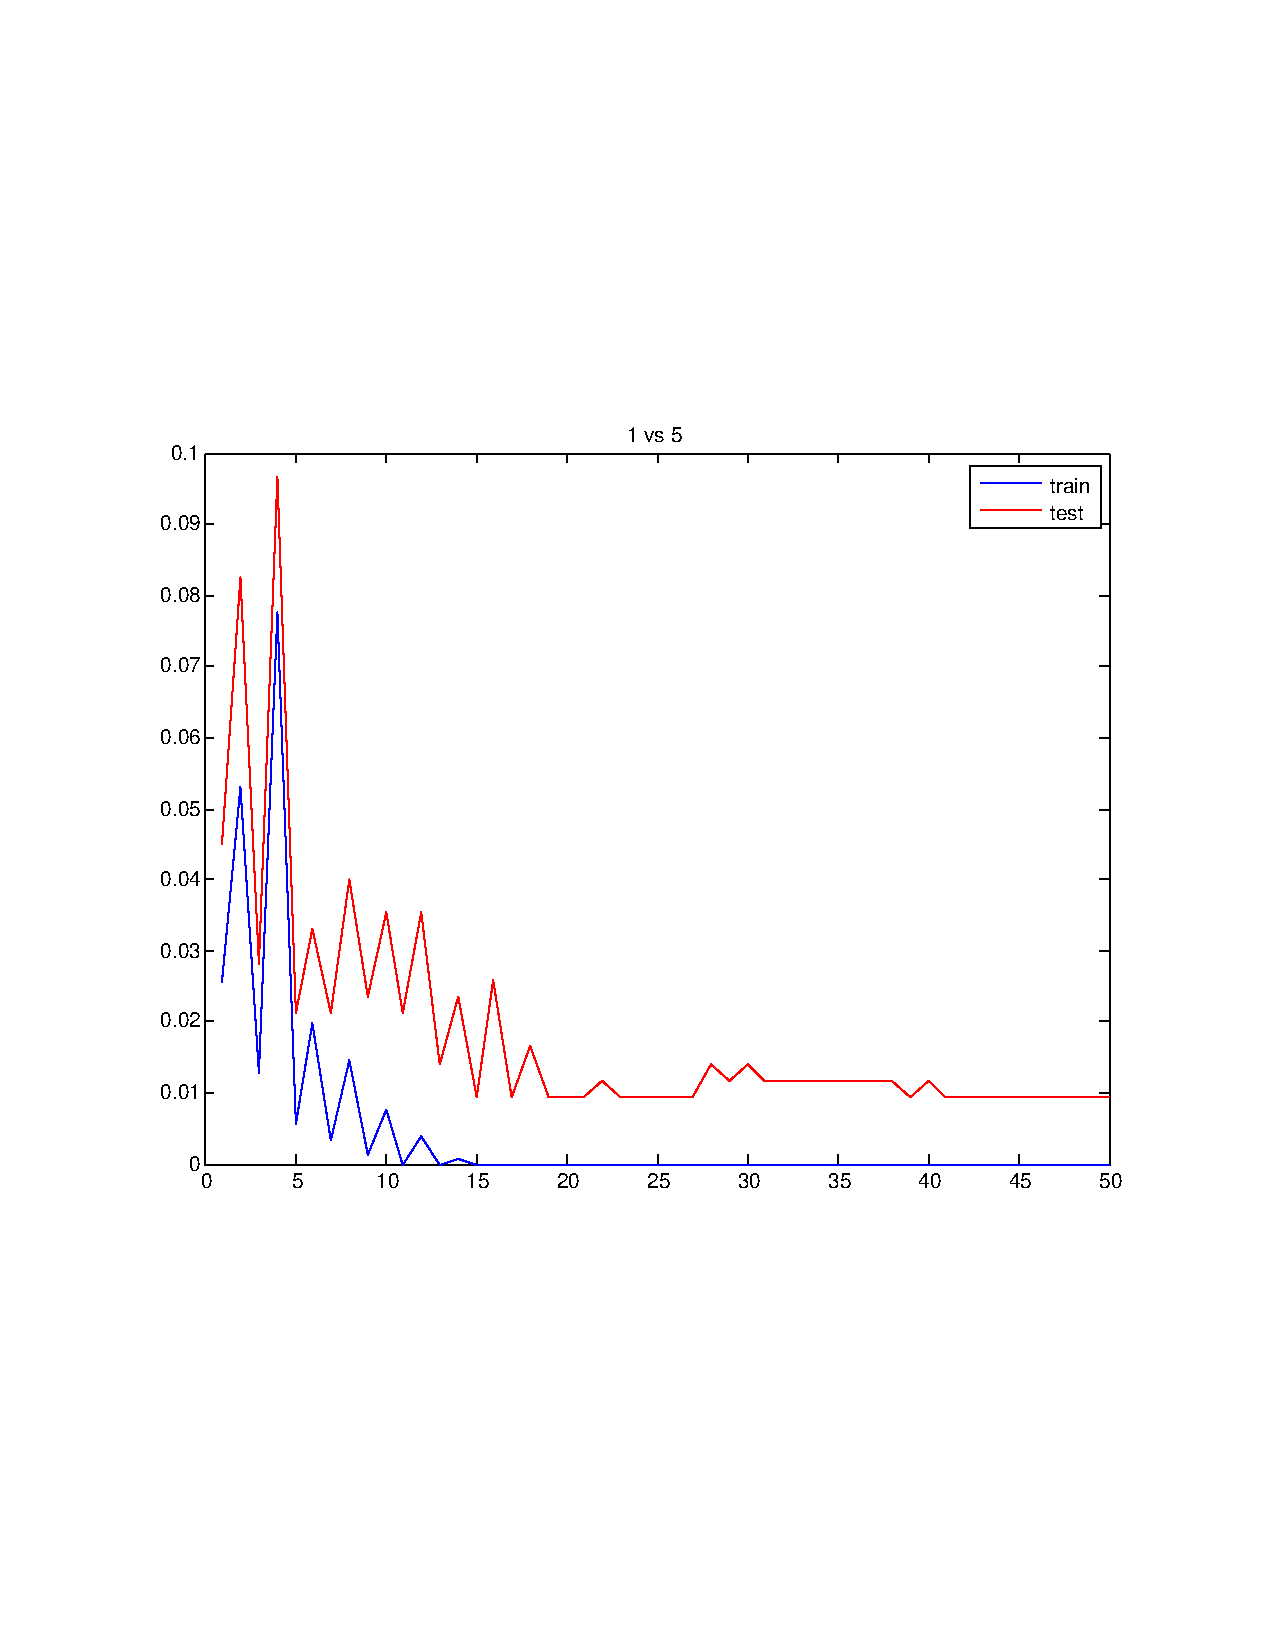
\includegraphics[width=.45\textwidth]{1v5fixed.pdf}
%        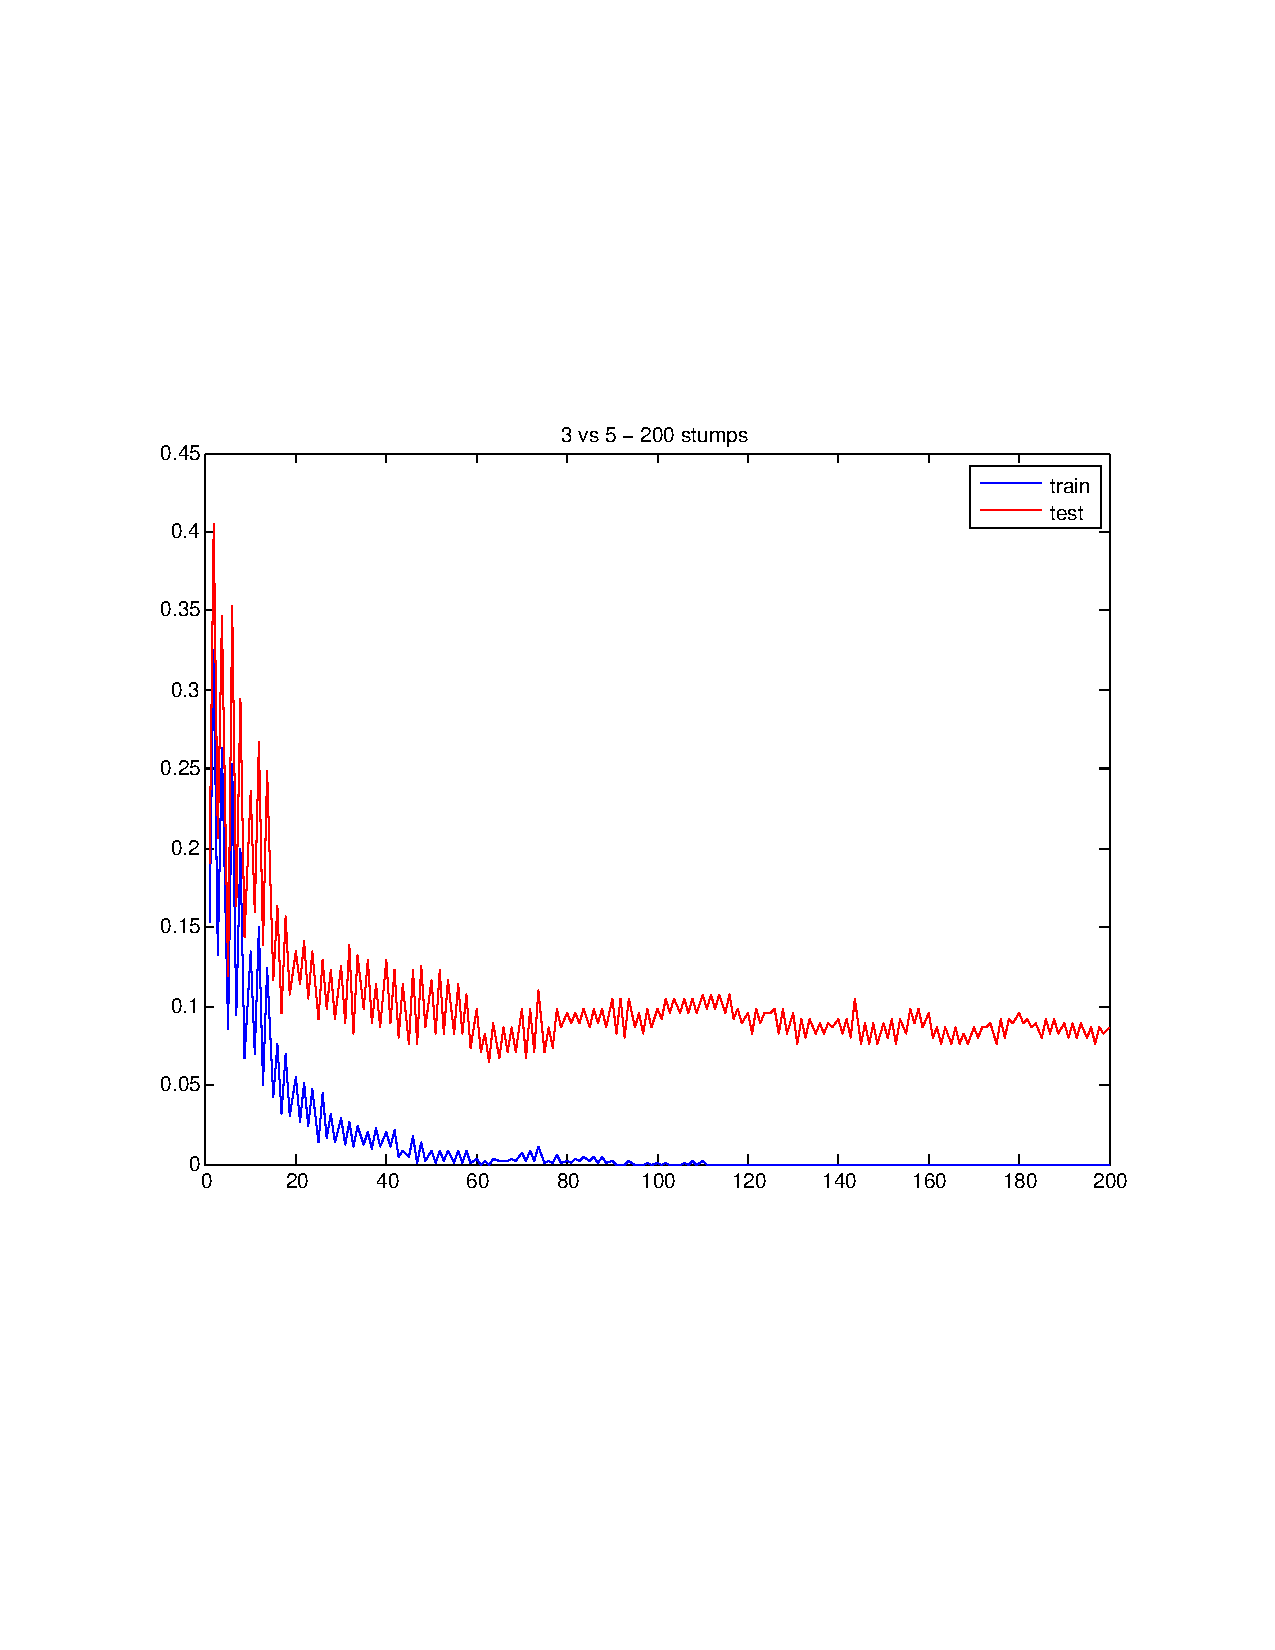
\includegraphics[width=.45\textwidth]{3v5_200.pdf}
%        \end{center}
%      \end{figure}
%

\end{enumerate}

\end{document}
